\section{LBO: lånefinansierade uppköp}
\label{sec:lbo}

\subsection{Hur en riskkapitalaffär fungerar}

Ett riskkapitalbolag \eng{private equity firm, financial sponsor} köper ett helt bolag, äger
det i några år och säljer det igen. Det speciella är finansieringen: en stor del av köpeskillingen
lånas, och lånen läggs på det köpta bolaget, som betalar ränta och amorteringar ur sitt eget
kassaflöde. Därav namnet \en{leveraged buyout}, LBO.

Varför låna? Ett räkneexempel. Ett bolag med EBITDA 100 köps för 1\,000 (10 gånger EBITDA),
med 600 i lån och 400 i eget kapital. Under fem år ger rörelsen 350 i kassaflöde före räntor.
Av det går 150 till ränta och 200 till amortering. EBITDA växer till 130, och bolaget säljs
till samma multipel, alltså för 1\,300. Skulden är då 400, och ägaren får $1\,300 - 400 = 900$.
Insatsen har vuxit 2,25 gånger, vilket är 17,6\pct{} om året. Utan lån hade ägaren satsat
1\,000 och fått $1\,300 + 350 = 1\,650$: 1,65 gånger pengarna, eller 10,5\pct{} om året. Samma
bolag, samma rörelse, men hävstången lyfter avkastningen på det egna kapitalet. Priset är
risken: om EBITDA faller i stället är det ägarens 400 som försvinner först.

\subsection{Källor och användning}

Varje affär börjar med en uppställning av var pengarna kommer ifrån och vad de används till
\eng{sources and uses}. De två sidorna ska vara lika, och ägarens insats är den post som får
det att gå ihop. Tabell~\ref{tab:sau} är motorns uppställning för Atlas Copco vid kurs plus
30\pct{} budpremie, alltså 249,93\kr{} per aktie.

\begin{table}[H]
\centering\small
\caption{Källor och användning för ett tänkt uppköp av Atlas Copco (mdkr).}
\label{tab:sau}
\begin{tabular}{@{}lrr@{\hspace{2.2em}}lrr@{}}
\toprule
Källor & mdkr & Andel & Användning & mdkr & Andel \\
\midrule
Seniort lån ($4,0 \times$ EBITDA) & 176,3 & 13,7\pct & Köp av aktierna & 1\,219,7 & 94,5\pct \\
Efterställt lån ($1,5 \times$) & 66,1 & 5,1\pct & Lösen av befintlig skuld & 37,5 & 2,9\pct \\
Bolagets egen kassa & 25,1 & 1,9\pct & Transaktionskostnader (2\pct{} av EV) & 24,6 & 1,9\pct \\
Ägarens insats & 1\,022,6 & 79,3\pct & Lånekostnader (2\pct{} av lånen) & 4,8 & 0,4\pct \\
 & & & Kassa som lämnas kvar & 3,4 & 0,3\pct \\
\midrule
Summa & 1\,290,1 & 100\pct & Summa & 1\,290,1 & 100\pct \\
\bottomrule
\end{tabular}
\end{table}

Redan här syns att affären är orealistisk: ägaren skulle behöva över 1\,000~mdkr, och priset
motsvarar 28,0 gånger EBITDA. Exemplet duger ändå för att visa mekaniken.

\subsection{Skuldtrancher}

Skulden delas i skikt \eng{tranches} med olika förmånsrätt, och ju längre bak i kön desto högre
ränta. Motorn har tre:

\begin{description}
  \item[Seniort lån] \eng{senior term loan}: 4,0 gånger EBITDA, ränta riskfri ränta plus 4
    procentenheter (7,075\pct), amorteras med 5\pct{} av ursprungsbeloppet per år och får
    dessutom all överskottskassa.
  \item[Efterställt lån] \eng{subordinated debt, mezzanine}: 1,5 gånger EBITDA, riskfri ränta
    plus 8 procentenheter (11,075\pct), betalas i sin helhet vid förfall \eng{bullet} och
    amorteras aldrig i förtid.
  \item[Checkkredit] \eng{revolving credit facility}: 0,5 gånger EBITDA, outnyttjad vid köpet,
    används bara om kassan inte räcker till ränta och amortering.
\end{description}

Lånen krymps vid behov så att tre villkor håller: EBITDA ska vara minst 2,0 gånger första
årets ränta, EBITDA minus capex minst 1,25 gånger ränta plus amortering, och ägarens insats
minst 30\pct{} av det nya kapitalet. Det efterställda lånet skärs först. Nivåerna (5,5 gånger
EBITDA, räntemarginalerna, 30\pct{} budpremie) är vanliga tumregler i läroböcker, inte
källbelagda marknadsdata.

\subsection{Kassaflödet och svepet}

Varje år går kassan genom en bestämd ordning, ett vattenfall. Överst står det kassaflöde som
finns att betala långivarna med: EBITDA minus skatt, capex och ökat rörelsekapital. Sedan
betalas ränta och obligatorisk amortering. Det som blir över, utöver en minsta kassa på 2\pct{}
av omsättningen, betalar först tillbaka checkkrediten och går sedan till extra amortering av
det seniora lånet. Det sista steget kallas \en{cash sweep}.

\begin{lstlisting}[caption={Vattenfallet i \texttt{\_project}, \texttt{models/lbo.py}
(förkortat).},label=lst:sweep]
cfads = ebitda - tax - capex - change_in_nwc
cash_interest = total_interest - sub_pik
mandatory = min(scheduled, senior)
excess_cash_flow = cfads - cash_interest - mandatory
surplus = cash + excess_cash_flow - minimum_cash
revolver_draw = min(max(-surplus, 0.0), max(revolver_limit - revolver, 0.0))
revolver_repayment = min(max(surplus, 0.0), revolver)
sweep = min(
    a.cash_sweep_pct * max(surplus - revolver_repayment, 0.0),
    senior - mandatory,
)
\end{lstlisting}

Två detaljer är värda att känna till. Räntan räknas på årets \emph{ingående} skuld, vilket gör
att modellen slipper cirkelreferensen mellan ränta och amortering som Excel-modeller brukar ha.
Och skatten räknas på EBIT minus avdragsgill ränta, där avdraget begränsas till 30\pct{} av
EBITDA, en förenkling av de svenska reglerna om ränteavdragsbegränsning. För Atlas Copco är
räntan första året 19,8~mdkr, men bara 14,1 får dras av.

\begin{figure}[ht]
\centering
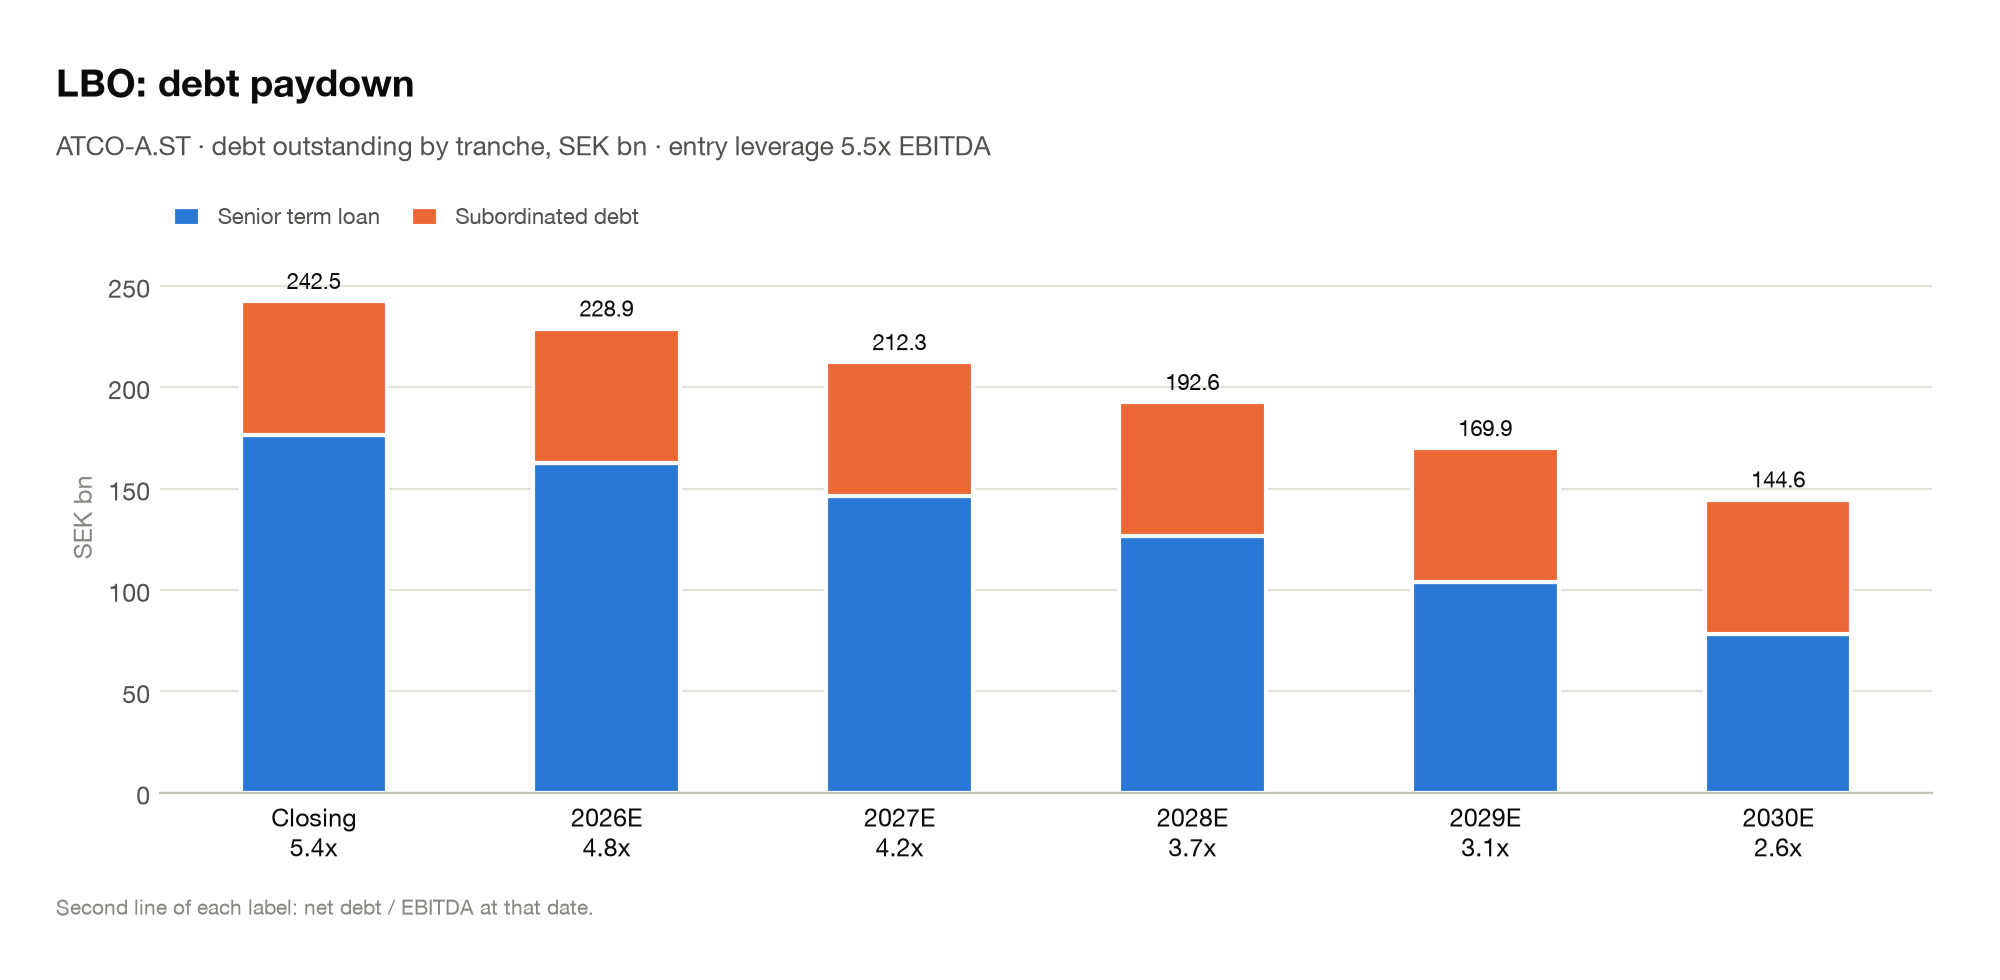
\includegraphics[width=0.92\linewidth]{lbo_debt_paydown.png}
\caption{Skulden år för år i motorns LBO på Atlas Copco. Det seniora lånet amorteras från 176
till 78~mdkr, det efterställda ligger kvar på 66.}
\label{fig:lbo-skuld}
\end{figure}

\subsection{Varifrån avkastningen kommer}
\label{sec:lbo-attribution}

Ägarens insats är köpets rörelsevärde plus avgifter minus nettoskulden efter köpet. Det ägaren
får vid försäljningen är rörelsevärdet då minus nettoskulden då. Skriv rörelsevärdet som
multipel gånger EBITDA, med index 0 för köpet och $x$ för försäljningen. Skillnaden blir
\begin{equation}
  {\underbrace{E_x - E_0}_{\text{värdeskapande}}}
  = {\underbrace{(\EBITDA_x - \EBITDA_0)\, M_0}_{\text{resultattillväxt}}}
  + {\underbrace{(M_x - M_0)\, \EBITDA_x}_{\text{multipelförändring}}}
  + {\underbrace{(\mathrm{ND}_0 - \mathrm{ND}_x)}_{\text{amortering}}}
  - \text{avgifter}.
  \label{eq:attribution}
\end{equation}
Identiteten följer av att
$M_x \EBITDA_x - M_0 \EBITDA_0 = (\EBITDA_x - \EBITDA_0) M_0 + (M_x - M_0)\EBITDA_x$. Det är de
tre källorna till avkastning som varje intervjuare vill höra: bolaget tjänar mer \eng{EBITDA
growth}, det säljs dyrare än det köptes \eng{multiple expansion}, och skulden har betalats
ned med bolagets egna pengar \eng{debt paydown, deleveraging}.

För Atlas Copco, köpt till 28,0 och sålt till 19,4 gånger EBITDA (figur~\ref{fig:lbo-vf}):
$278,5 - 460,7 + 98,6 - 29,5 = -113,1$~mdkr. Ägaren får tillbaka 909 av 1\,023~mdkr.
Resultattillväxt och amortering räcker inte när multipeln faller så mycket.

\begin{figure}[ht]
\centering
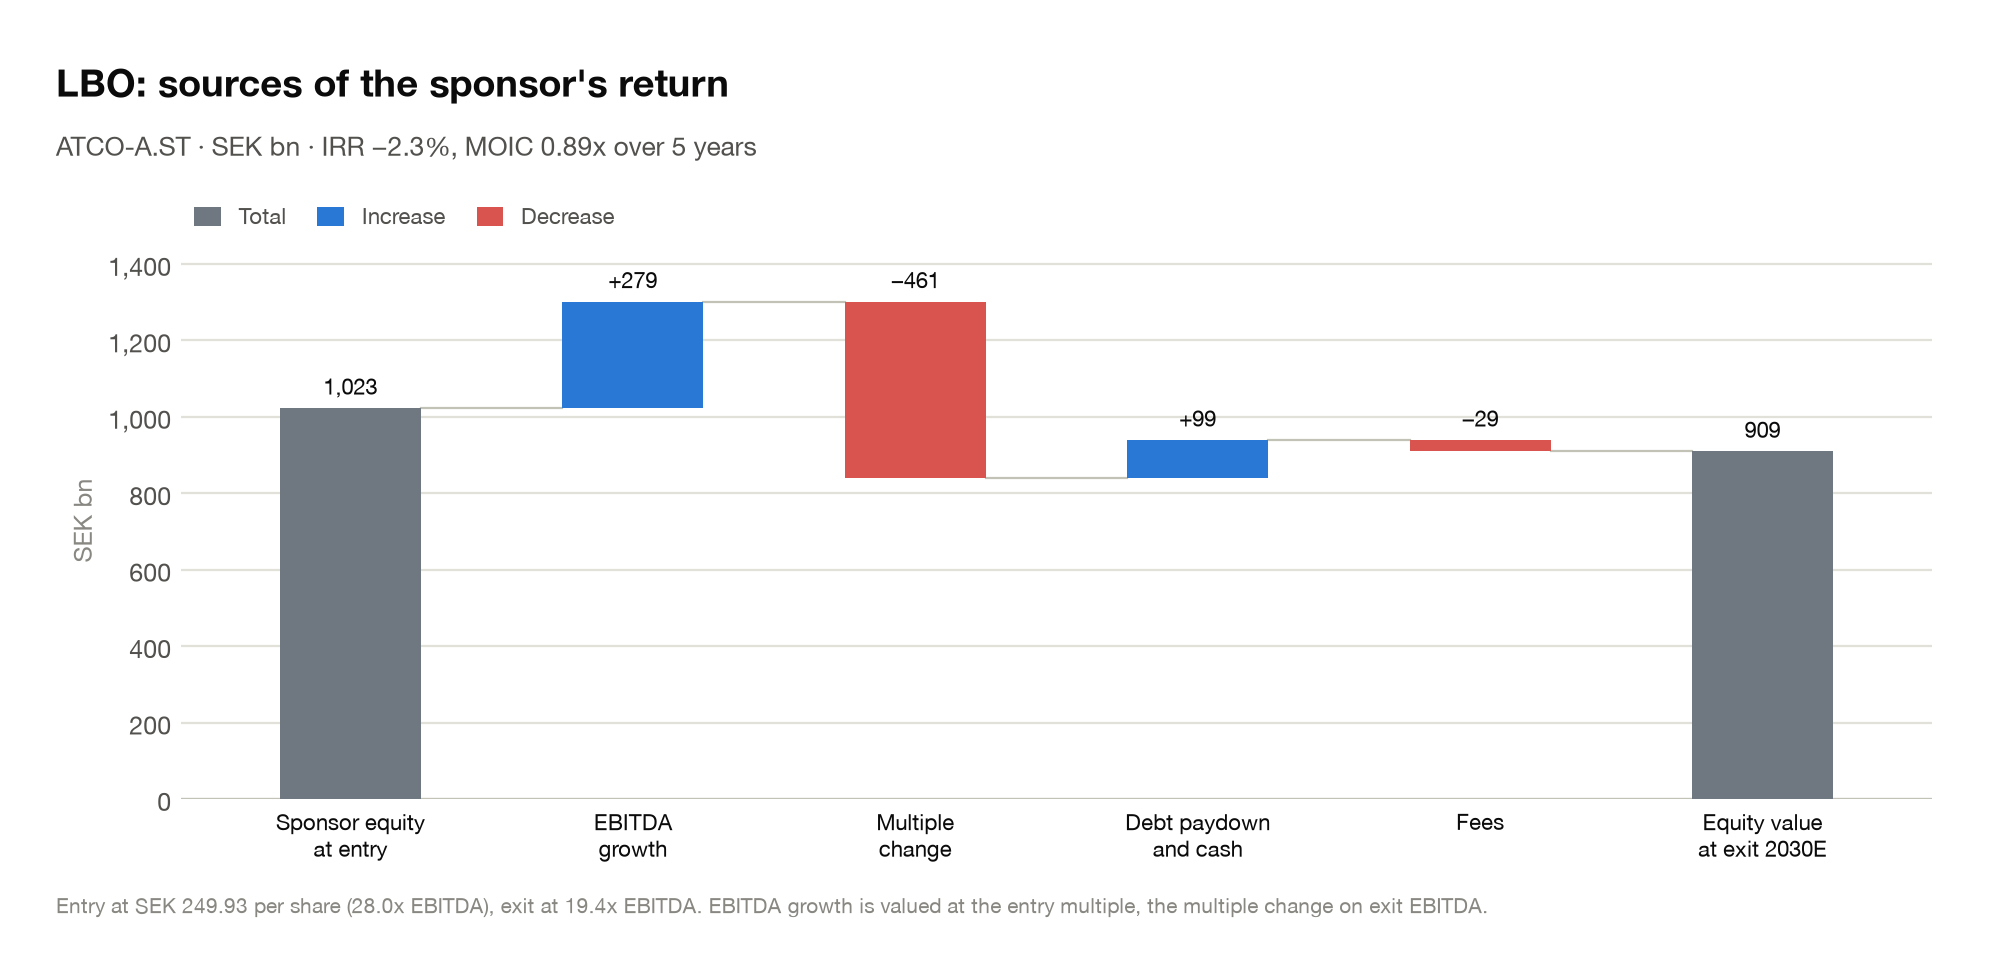
\includegraphics[width=0.92\linewidth]{lbo_returns_waterfall.png}
\caption{Uppdelningen~\eqref{eq:attribution} för Atlas Copco vid kurs plus 30\pct{} premie.}
\label{fig:lbo-vf}
\end{figure}

\subsection{IRR och MOIC}

Två mått används. MOIC \eng{multiple on invested capital} är pengar ut delat med pengar in.
IRR, internräntan \eng{internal rate of return}, är den ränta som gör nuvärdet av ägarens
alla kassaflöden $C_0, \dots, C_N$ till noll:
\begin{equation}
  \sum_{t=0}^{N} \frac{C_t}{(1+\IRR)^t} = 0 .
  \label{eq:irr}
\end{equation}

\paragraph{IRR som rot till ett polynom.} Sätt $x = 1/(1+\IRR)$. Då är~\eqref{eq:irr} ekvationen
$p(x) = \sum_t C_t x^t = 0$, ett polynom av grad $N$, och vi söker rötter med $x > 0$. Tre
saker är värda att kunna:

\begin{itemize}
  \item \textbf{Existens och entydighet.} Om kassaflödena byter tecken exakt en gång (först en
    insats, sedan bara inflöden) har $p$ enligt Descartes teckenregel exakt en positiv rot. Då
    finns precis en internränta över $-100$\pct.
  \item \textbf{Flera rötter.} Med flera teckenbyten kan det finnas flera. Flödena
    $-100, +230, -132$ ger $100(1+r)^2 - 230(1+r) + 132 = 0$ med rötterna $r = 10$\pct{} och
    $r = 20$\pct. Motorns \kod{compute_irr} returnerar då den minsta.
  \item \textbf{Varför rotsökning.} För grad fem och högre finns ingen allmän lösningsformel
    (Abel och Ruffini), så internräntan måste sökas numeriskt. Motorn använder Brents metod
    (\kod{scipy.optimize.brentq}), som kombinerar intervallhalvering med interpolation och
    alltid konvergerar när funktionen byter tecken på intervallet.
\end{itemize}

I motorns LBO finns inga utdelningar under innehavet, så ägarens flöden är bara insatsen och
försäljningen. Då har~\eqref{eq:irr} en sluten lösning:
\begin{equation}
  \IRR = \MOIC^{1/N} - 1 .
  \label{eq:irr-moic}
\end{equation}
För Atlas Copco: $\MOIC = 909/1\,023 = 0,89$ och $\IRR = 0,89^{1/5} - 1 = -2,3$\pct{} om året.

\begin{komihag}
MOIC säger hur mycket, IRR säger hur fort. Dubbla pengarna på tre år är 26\pct{} om året, på
fem år 15\pct. Tre gånger pengarna på fem år är 25\pct. En fond som säljer tidigt kan visa hög
IRR med låg MOIC, och därför tittar investerare på båda.
\end{komihag}

\subsection{Betalningsförmåga: LBO som värderingsmetod}

Till football field behövs ett pris, inte en avkastning. Motorn vänder därför på frågan: vilket
pris per aktie $P$ kan en riskkapitalköpare betala och ändå nå sitt avkastningskrav? Det kallas
\en{ability to pay}. Motorn söker roten till
\begin{equation}
  f(P) = -E_0(P) + \frac{E_x(P)}{(1 + \IRR^{*})^N} = 0,
  \label{eq:atp}
\end{equation}
där $E_0(P)$ är insatsen och $E_x(P)$ försäljningslikviden vid priset $P$. Här behövs
rotsökningen på riktigt, eftersom lånevillkoren gör $E_0$ och $E_x$ till styckvis definierade
funktioner av $P$. Stapelns ändar är tre avkastningskrav: 25\pct{} ger det låga priset,
20\pct{} basvärdet och 15\pct{} det höga. Kraven är vanliga tumregler för vad riskkapitalfonder
siktar på.

För Atlas Copco blir priserna 104,4, 117,9 och 135,3\kr. Vid 117,9\kr{} motsvarar köpet 13,3
gånger EBITDA, insatsen är 60\pct{} av det nya kapitalet och pengarna växer 2,49 gånger på fem
år, vilket är exakt 20\pct{} om året. Lånen är desamma som i tabell~\ref{tab:sau}, eftersom de
bestäms av EBITDA och inte av priset. Lägre pris betyder därför mindre eget kapital och högre
hävstång.

\begin{intervjutips}
En LBO-värdering kallas ofta ett golv \eng{floor valuation}: en finansiell köpare har inga
synergier och ett högt avkastningskrav, så en industriell köpare bör kunna betala mer. Lägg
märke till att LBO-värdet i caset (118\kr) hamnar nära Gordon-DCF:en (116\kr). Det är samma
kassaflöden, värderade med 20\pct{} avkastningskrav och lånefinansiering till hjälp i stället
för 7,65\pct{} utan.
\end{intervjutips}
